\documentclass{ctexart}[UTF-8]        %中文article文档类型排版,UTF8编码
\usepackage{amsmath}                 %调用公式宏包
\usepackage{graphicx}                %插入图片宏包
\usepackage{hyperref}
\usepackage{fontspec}
\hypersetup{
            colorlinks,
            linkcolor=red,
            anchorcolor=blue,
            citecolor=green,
            CJKbookmarks=True
            }




\newtheorem{thm}{定理}               %定义标题为定理的定理类环境thm
\newcommand\degree{^\circ}           %定义新命令degree用来写角度的



\begin{document}



\title{Influence of Thickness and Contact Area on the Performance of PDMS-Based Triboelectric Nano generators \\ [2ex] \small 厚度和接触面积对基于PDMS的摩擦纳米发电机性能的影响}
\author{史学睿}
\date{\today}
\maketitle



%摘要
\begin{abstract}
    摩擦电层的厚度和两摩擦电材料之间的接触面积对电信号的影响。使用了PDMS-尼龙摩擦对,
    并改变PDMS层的厚度。厚度增加,电压降低;但是最大电流,却随之升高。摩擦电层厚度为32um时,
    输出功率最大,然后急剧降低。增大接触面积,提高电输出。
\end{abstract}

%第一节
\section{简介}

摩擦纳米发电机分为四种:垂直接触分离(vertical contact-separation)、侧向滑动(lateral-sliding)、
单电极(single-electrode)和独立式摩擦电层(freestanding triboelectric-layer)。

闭合电路的输出电压为:

\begin{equation}
    V = - \frac{Q}{A \varepsilon_0}[d_0+x(t)]+ \frac{\sigma x(t)}{\varepsilon_0}
\end{equation}

开路电压为:

\begin{equation}
    V_{OC} = \frac{\sigma x(t)}{\varepsilon_0}
\end{equation}

其中,Q是转移电荷量

x(t)是两电极之间的时间距离关系

$\varepsilon_0$是真空介电常数

$d_0$是两电极之间的有效长度,由$\frac{d_1}{\varepsilon_{r1}} + \frac{d_2}{\varepsilon_{r2}} $给出

TENG产生的短路电流与摩擦电荷密度($\sigma$),电极面积(A),和相对机械运动速度$v(t)$
成正比,与电极之间距离的平方成反比:

\begin{equation}
    I_{SC} = \frac{\sigma A d_0 v(t)}{[d_0 + x(t)]^2}
\end{equation}

PDMS由于其柔韧性,易于制造,生物相容性和超疏水性而被广泛使用。

尼龙具有良好的机械性能(强度和刚度),高抗冲击性,易于制造并且在较大的温度范围能能保持其性能。

%第二节
\section{实验细节}

实验材料:

SYLGARD 182 硅胶弹性体套件,由两部分组成,包括PDMS基底和固化剂(二甲基,甲基氢硅氧烷)
,基底和固化剂的质量比为10:1。

利用旋涂技术将PDMS沉积在铝基板上用作一个电极。旋涂速度从 500到5000 rpm变化,
使得PDMS层的厚度在13到220 $\mu$m 之间,然后将PDMS在80℃的恒温箱中固化两小时。
另一种摩擦材料(尼龙)作为厚度为50$\mu$m的薄膜使用。在两材料上都缠上铝胶带作为电极,
并放入(20$cm^2$)的丙烯酸板中。使用100到1G$\Omega$电阻的电路测量电流、电压和功率与负载的关系。


%第三节
\section{结果和讨论}

PDMS厚度为$13\mu m$时,电压为1.4V最大;厚度为$220\mu m$时,电压为0.2V最小。
与PDMS薄膜的固有特性相关,例如刚度、硬度或粗糙度及其厚度相关。电流的饱和值约为1.3$\mu A$
这些结果与纳米摩擦发电机的理论相一致。然后是负载为100到1$G\Omega$的电压和电流。结果表明,
对于所有的样品,在负载超过$10K\Omega$时,电压趋于恒定值(开路电压)。而电流的变化正相反。
结果表明,在PDMS层厚度为32$\mu m$时,功率最大为0.56$\mu W$,对应的功率密度为0.55$mW/m^2$
最小值为0.23$\mu W$,对应的功率密度为0.23$mW/m^2$.


\begin{figure}[!ht]\centering
    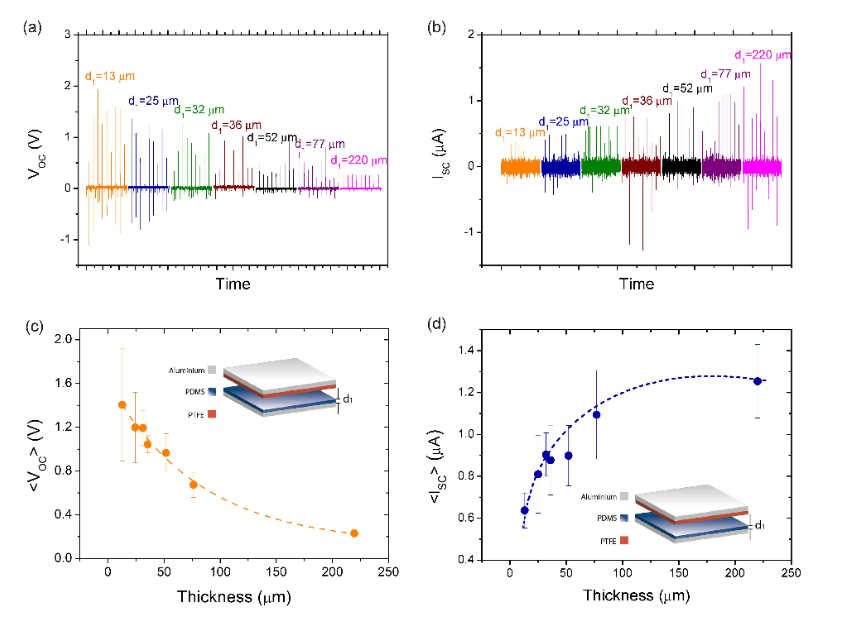
\includegraphics[width=0.80\textwidth]{Image/V-I.png}
    \caption{实验结果}
\end{figure}



\begin{figure}[!ht]\centering
    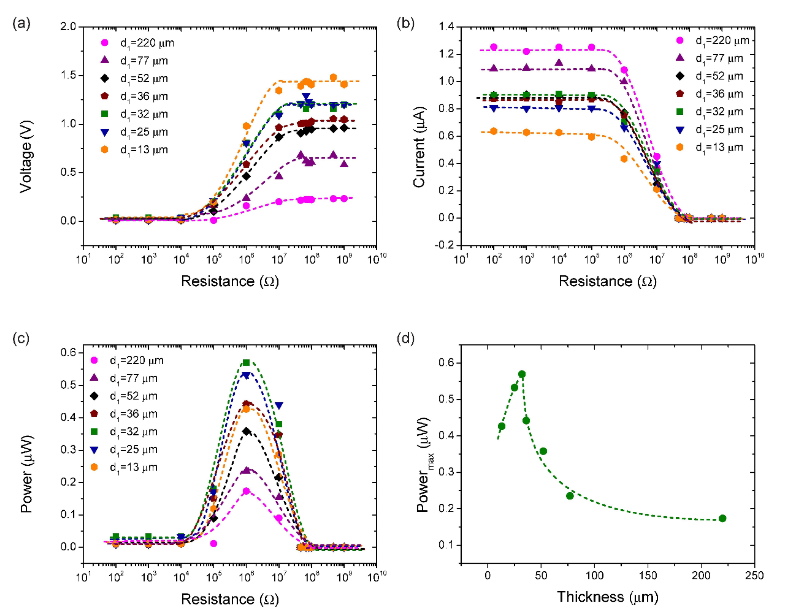
\includegraphics[width=0.80\textwidth]{Image/R-P.png}
    \caption{实验结果}
\end{figure}


\subsection{摩擦电层面积的影响}

面积从2.5到15$cm^2$变化,使用PDMS-尼龙摩擦对,PDMS层厚度为32$\mu m$
开路电压、短路电流和输出电流都随着面积的增大而增大。计算了不同面积的电压和电流峰值的平均值。
图三显示了在垂直接触分离模式下PDMS-尼龙摩擦对产生的开路电压的平均值。面积为15$cm^2$
时电压达到最大值为1.2V,电流达到最大值为0.34$\mu A$。随着接触面积的增大,输出电压和电流均随之增大。
对这四种面积在负载为100到1$G\Omega$时分别测量电学输出,如预期相同,高电阻下电压有最大值1.2V,
在小电阻下电流达到最大值0.43$\mu A$。随着面积的增大,最大输出功率也随之增加,可达到
0.5$\mu W$,相应的功率密度为0.33$mW/m^2$。


\begin{figure}[!ht]\centering
    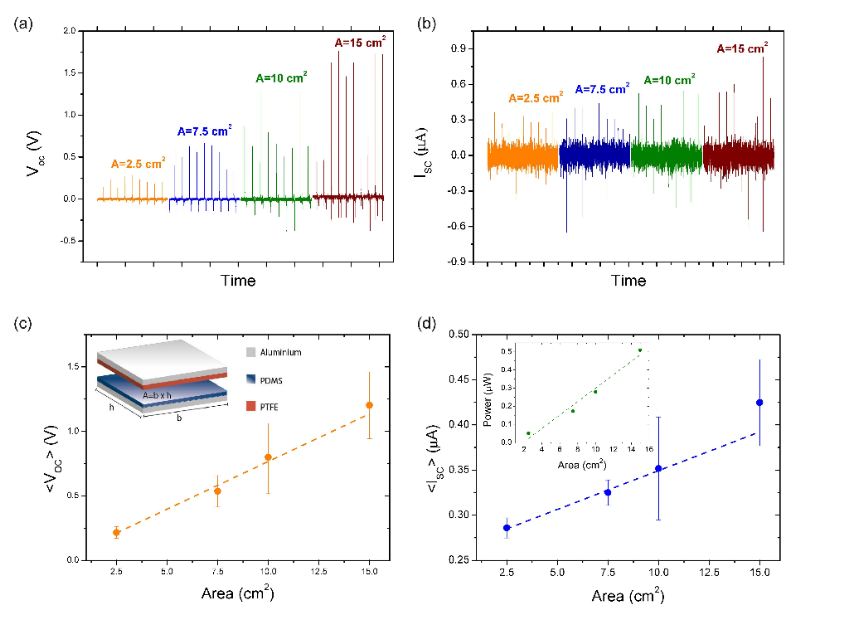
\includegraphics[width=0.80\textwidth]{Image/V-S.png}
    \caption{实验结果}
\end{figure}


\end{document}